% Quick start guide
\documentclass{beamer}

\usetheme {default}

% Title page details
\title{Varroa mites causing Colony Collapse Disorder CCD}
\author{By:Julia Almeida, Kimberly Ortiz}
\institute{Institue for Computing in Research}
\date{August 2, 2023}

\begin{document}

\setbeamertemplate{background}
{

\includegraphics[width=20cm, height=15cm]{mites.jpg}
}

\begin{frame}
% Print the title page as the first slide
  \titlepage
\end{frame}

% ...
% Lists in beamer (Itemize)
\begin{frame}{Outline}{\large}
\begin{itemize}
    \item 1.Introduction
    \item 2.Background
    \item 3.Process
    \item 4.Results
    \item 5.Future Work
    \item 6.Refrences
\end{itemize}
\end{frame}

\begin{frame}
  \frametitle{Main Objective}
  \begin{itemize}
  \item How can we model the Colony Collapse in honey bees?
  \item How can we prevent or find a solution?
  \end{itemize}
\end{frame}

\begin{frame}
  \frametitle{Varroa Virus}
What is Varroa virus?
\linebreak
External parasites that attack honey bees directly and indirectly

  Direct Attack
  \begin{itemize}
  \item Attach directly into the bees abdomen and begin sucking the blood
  \end{itemize}

  Indirectly Attack
  \begin{itemize}
  \item Transmit other pathogenic viruses
  \end{itemize}
\end{frame}

\begin{frame}
  \frametitle{DNA vs. RNA}

  \begin{figure}
  \centering
      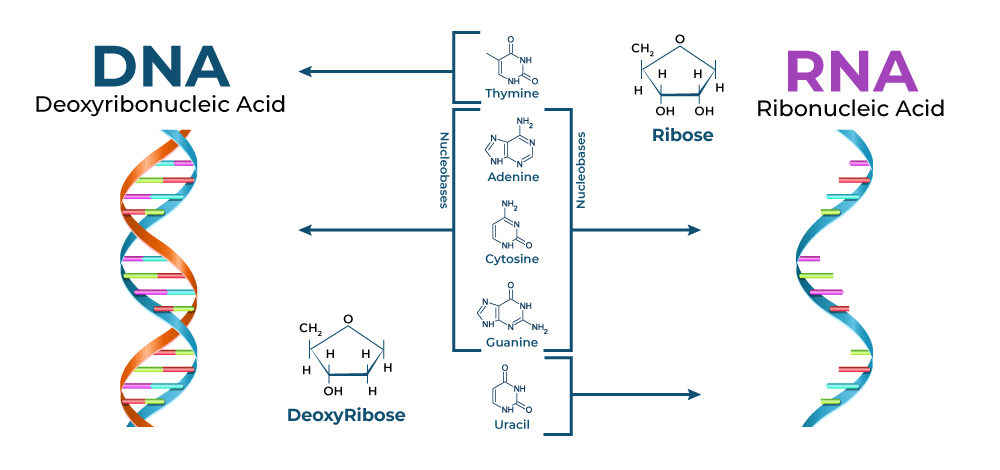
\includegraphics[width=10cm]{DNA-vs-RNA.png}
      \caption{Differences between DNA \& RNA}
      \label{DNA&RNA}
  \centering 
  \end{figure}
\end{frame}

\begin{frame}
  \frametitle{Development Stages}

  \begin{figure}
  \centering
      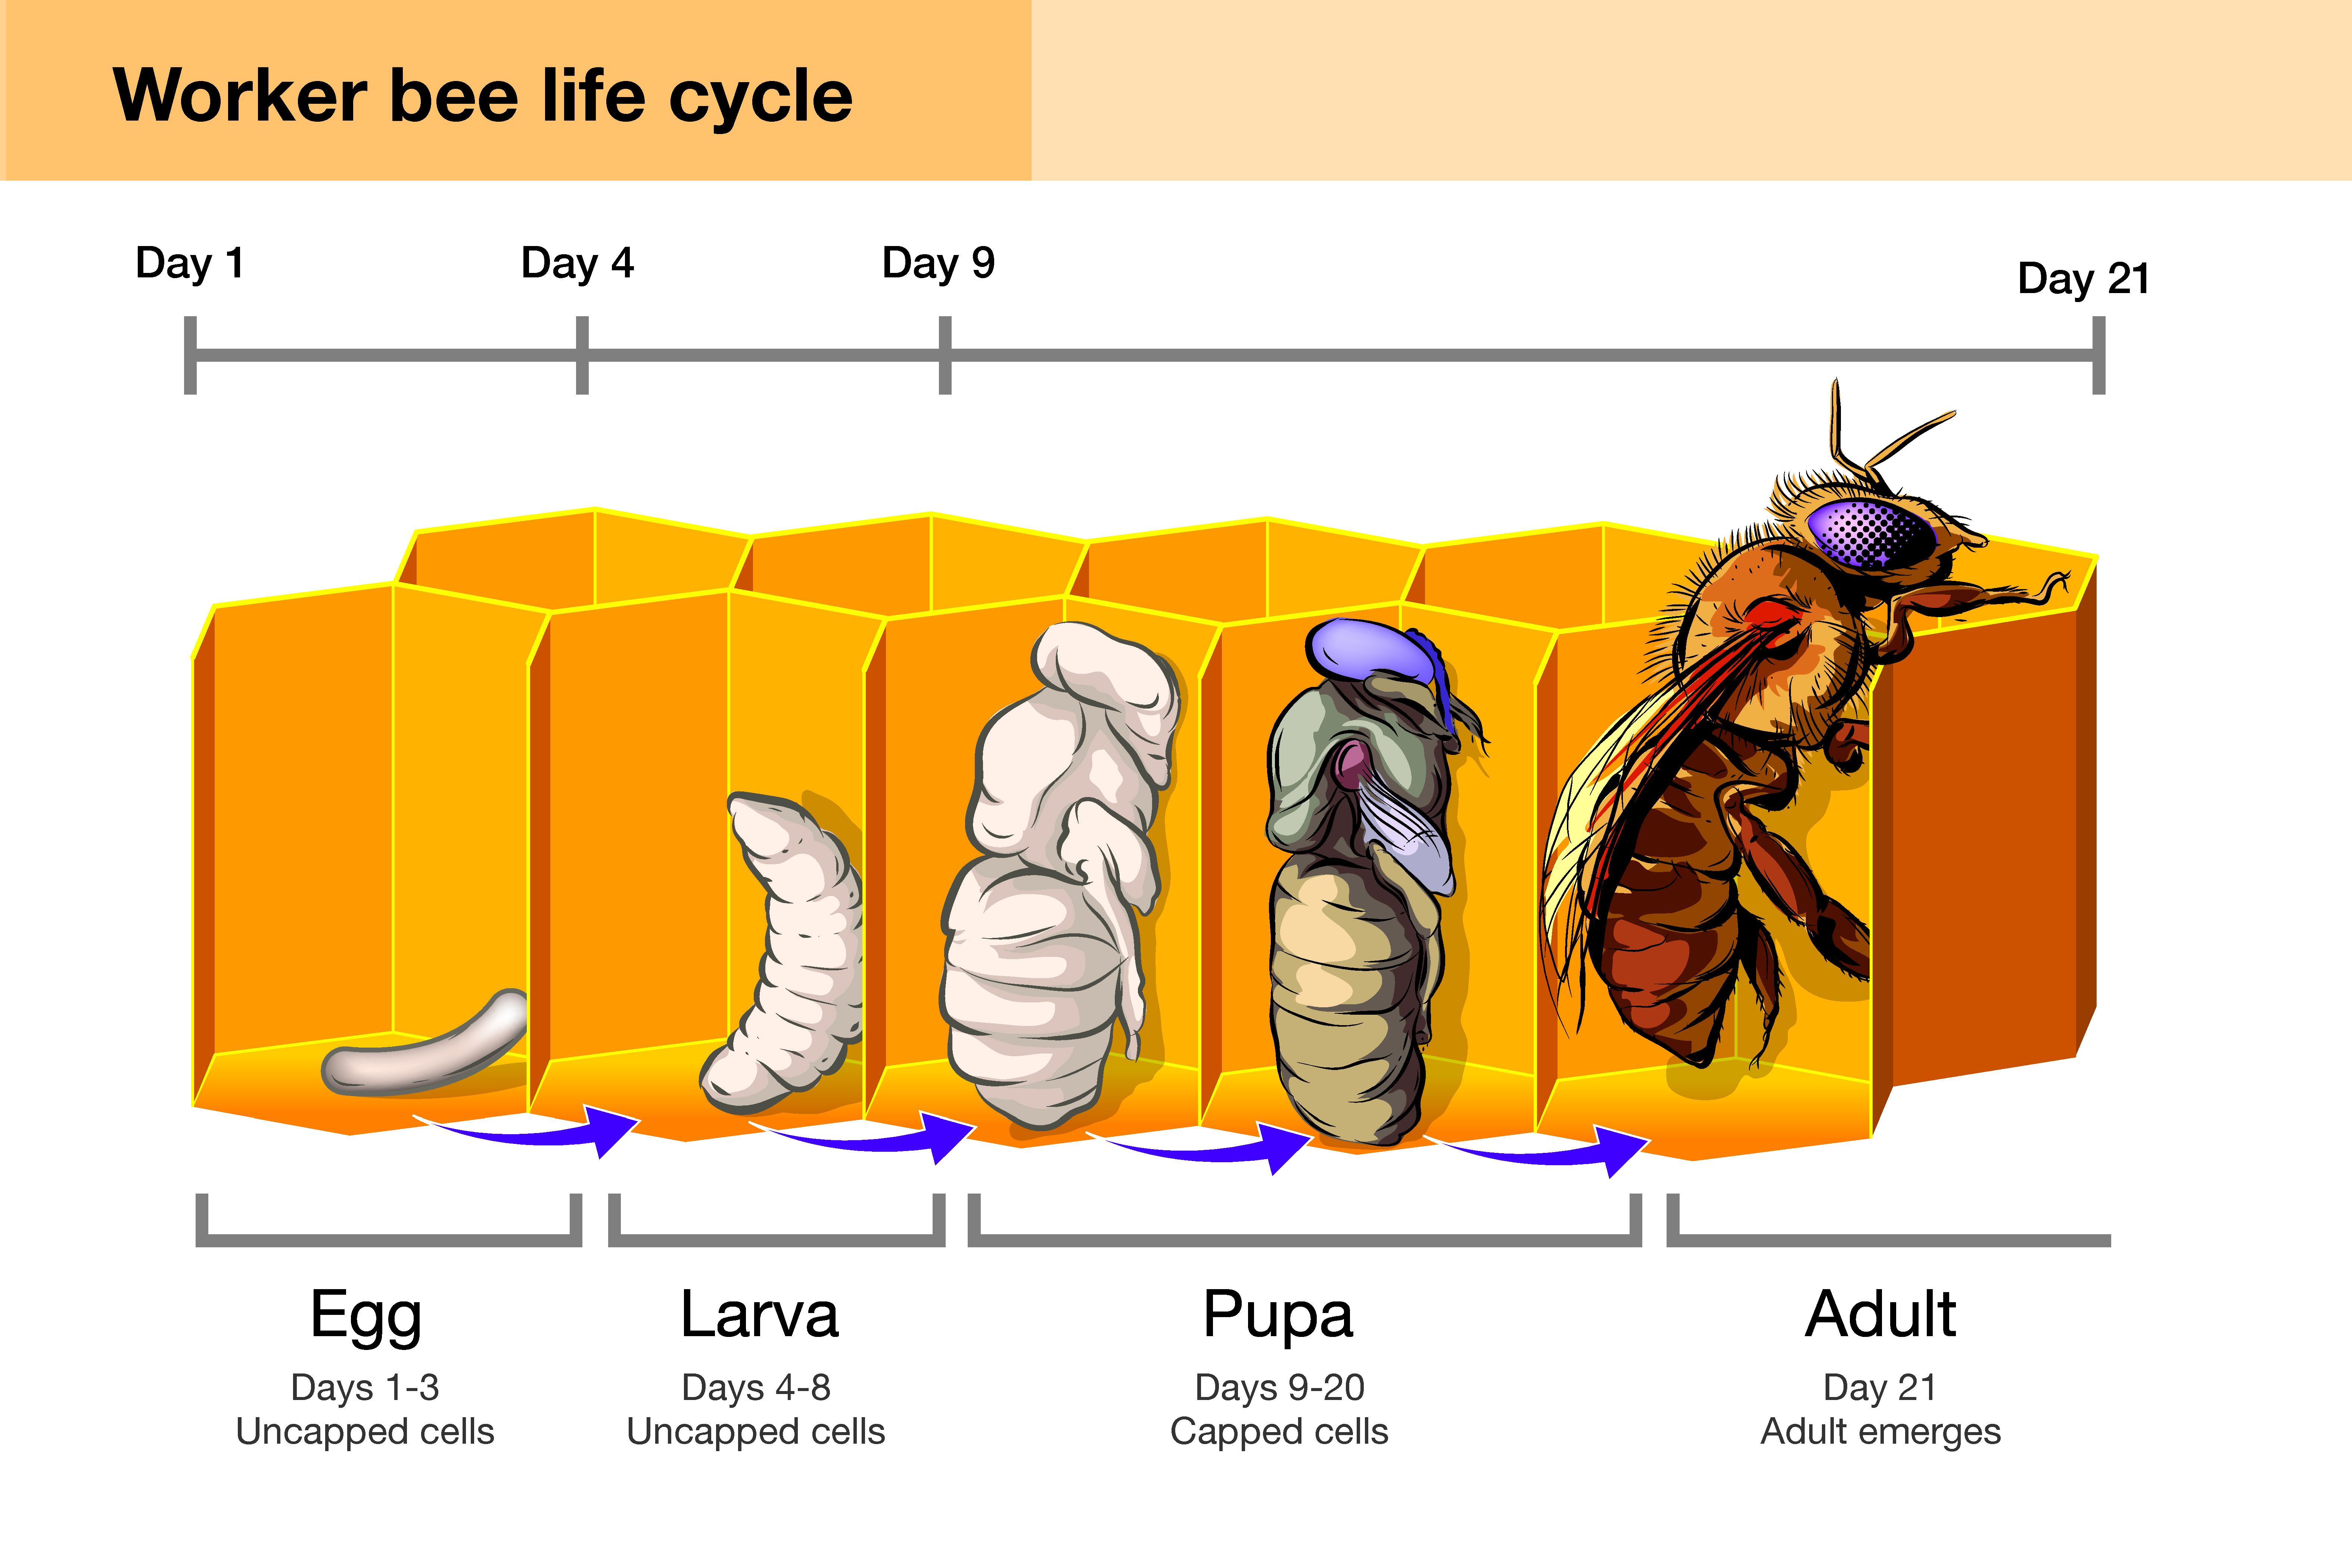
\includegraphics[width=9cm]{LifeCycle_Page_1.jpg}
      \caption{Life Cycle of a Honey Bee}
      \label{Life Cycle}
  \centering
  \end{figure}
\end{frame}


\begin{frame}
  \frametitle{Simulation}
  \begin{figure}
    \centering
    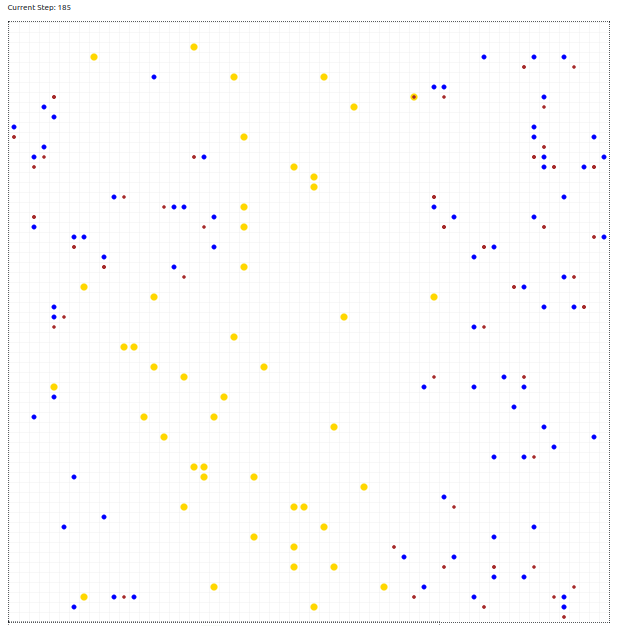
\includegraphics[width=8cm]{bees_model_pic.png}
    \caption{Agent-Based Model}
    \label{Agent-Based Model}
    \centering
  \end{figure}
  

\end{frame}

\begin{frame}
  \frametitle{Graph}
  \begin{figure}
  \centering
    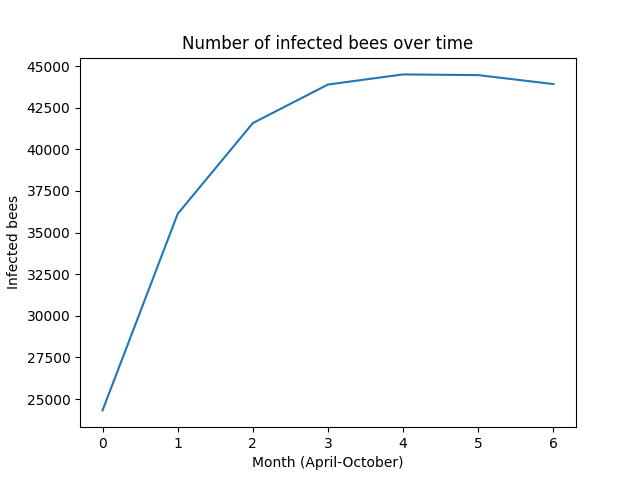
\includegraphics[width=10cm]{Figure_2.png}
    \caption{Infection Rate}
    \label{Infection Rate}
  \centering
  \end{figure}
\end{frame}

\begin{frame}
  \frametitle{CRISPR}
  \begin{itemize}
  \item CRISPR is designed to guide RNA to deliver reagents and allow repair to occur
  \end{itemize}
\end{frame}

\begin{frame}
  \frametitle{How we are using CRISPR}
  \begin{figure}
  \centering
    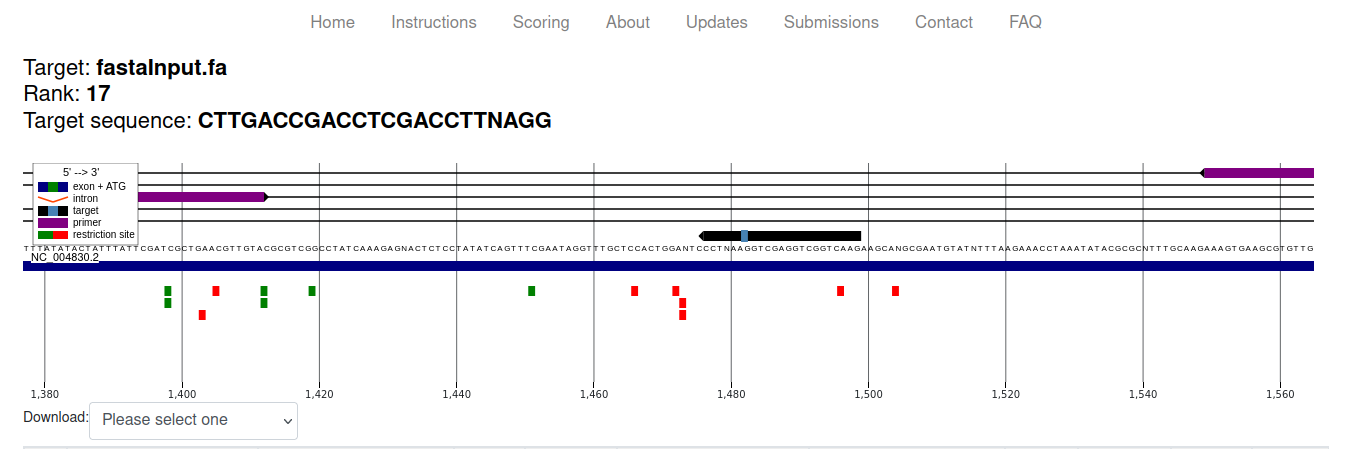
\includegraphics[width=10.5cm]{VirusSequence.png}
    \caption{CHOP CHOP Varroa virus Genetic Sequence}
    \label{CHOP CHOP}
  \centering
  \end{figure}
\end{frame}

\begin{frame}
  \frametitle{Future Work}
  \begin{itemize}
  \item Compare different seasons and see how they assimilate or differ
  \item Explore CRISPR and new methods that might help prevent CCD
  \item Compare the genetics of bees in different regions
  \end{itemize}
  
\end{frame}

\begin{frame}
  \frametitle{Refrences}

\end{frame}

\begin{frame}
Thank you!
Questions?
\end{frame}

\end{document}
